\documentclass[border = 3mm]{standalone}

\renewcommand{\familydefault}{\sfdefault} % Sans serif default

\usepackage{tikz}
\usepackage{adjustbox}
\usetikzlibrary{patterns.meta}

\begin{document}
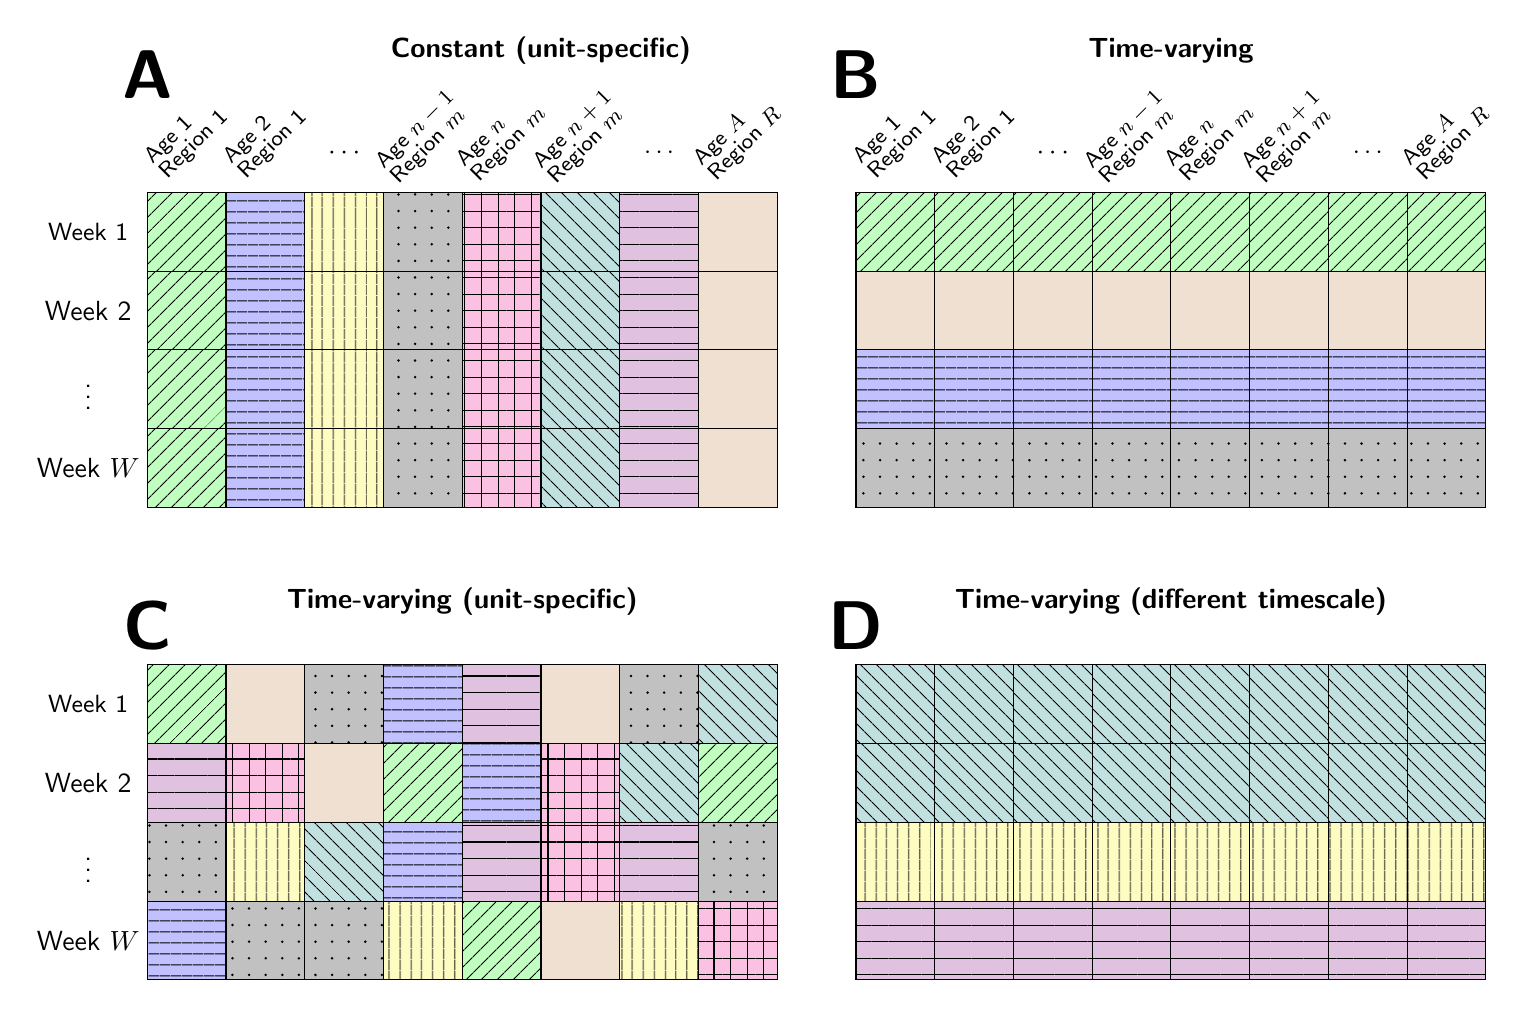
\begin{tikzpicture}
	%%A
	% Top row
	\draw [preaction = {fill = white!20!green, fill opacity = 0.3}, pattern = {Lines[angle = 45, distance = 4pt]}] (0, 3) rectangle (1, 4);
	\draw [preaction = {fill = white!20!blue, fill opacity = 0.3}, pattern = {Lines[distance = 4pt]}] (1, 3) rectangle (2, 4);
	\draw [preaction = {fill = white!20!yellow, fill opacity = 0.3}, pattern = {Lines[angle = 90, distance = 4pt]}] (2, 3) rectangle (3, 4);
	\draw [preaction = {fill = white!20!black, fill opacity = 0.3}, pattern = {Dots[distance = 6pt]}] (3, 3) rectangle (4, 4);
	\draw [preaction = {fill = white!20!magenta, fill opacity = 0.3}, pattern = {Hatch[distance = 6pt]}] (4, 3) rectangle (5, 4);
	\draw [preaction = {fill = white!20!teal, fill opacity = 0.3}, pattern = {Lines[angle = 135, distance = 4pt]}] (5, 3) rectangle (6, 4);
	\draw [preaction = {fill = white!20!violet, fill opacity = 0.3}, pattern = {Lines[distance = 6pt]}] (6, 3) rectangle (7, 4);
	\draw [preaction = {fill = white!20!brown, fill opacity = 0.3}] (7, 3) rectangle (8, 4);
	% Second row
	\draw [preaction = {fill = white!20!green, fill opacity = 0.3}, pattern = {Lines[angle = 45, distance = 4pt]}] (0, 2) rectangle (1, 3);
	\draw [preaction = {fill = white!20!blue, fill opacity = 0.3}, pattern = {Lines[distance = 4pt]}] (1, 2) rectangle (2, 3);
	\draw [preaction = {fill = white!20!yellow, fill opacity = 0.3}, pattern = {Lines[angle = 90, distance = 4pt]}] (2, 2) rectangle (3, 3);
	\draw [preaction = {fill = white!20!black, fill opacity = 0.3}, pattern = {Dots[distance = 6pt]}] (3, 2) rectangle (4, 3);
	\draw [preaction = {fill = white!20!magenta, fill opacity = 0.3}, pattern = {Hatch[distance = 6pt]}] (4, 2) rectangle (5, 3);
	\draw [preaction = {fill = white!20!teal, fill opacity = 0.3}, pattern = {Lines[angle = 135, distance = 4pt]}] (5, 2) rectangle (6, 3);
	\draw [preaction = {fill = white!20!violet, fill opacity = 0.3}, pattern = {Lines[distance = 6pt]}] (6, 2) rectangle (7, 3);
	\draw [preaction = {fill = white!20!brown, fill opacity = 0.3}] (7, 2) rectangle (8, 3);
	% Third row
	\draw [preaction = {fill = white!20!green, fill opacity = 0.3}, pattern = {Lines[angle = 45, distance = 4pt]}] (0, 1) rectangle (1, 2);
	\draw [preaction = {fill = white!20!blue, fill opacity = 0.3}, pattern = {Lines[distance = 4pt]}] (1, 1) rectangle (2, 2);
	\draw [preaction = {fill = white!20!yellow, fill opacity = 0.3}, pattern = {Lines[angle = 90, distance = 4pt]}] (2, 1) rectangle (3, 2);
	\draw [preaction = {fill = white!20!black, fill opacity = 0.3}, pattern = {Dots[distance = 6pt]}] (3, 1) rectangle (4, 2);
	\draw [preaction = {fill = white!20!magenta, fill opacity = 0.3}, pattern = {Hatch[distance = 6pt]}] (4, 1) rectangle (5, 2);
	\draw [preaction = {fill = white!20!teal, fill opacity = 0.3}, pattern = {Lines[angle = 135, distance = 4pt]}] (5, 1) rectangle (6, 2);
	\draw [preaction = {fill = white!20!violet, fill opacity = 0.3}, pattern = {Lines[distance = 6pt]}] (6, 1) rectangle (7, 2);
	\draw [preaction = {fill = white!20!brown, fill opacity = 0.3}] (7, 1) rectangle (8, 2);
	% Bottom row
	\draw [preaction = {fill = white!20!green, fill opacity = 0.3}, pattern = {Lines[angle = 45, distance = 4pt]}] (0, 0) rectangle (1, 1);
	\draw [preaction = {fill = white!20!blue, fill opacity = 0.3}, pattern = {Lines[distance = 4pt]}] (1, 0) rectangle (2, 1);
	\draw [preaction = {fill = white!20!yellow, fill opacity = 0.3}, pattern = {Lines[angle = 90, distance = 4pt]}] (2, 0) rectangle (3, 1);
	\draw [preaction = {fill = white!20!black, fill opacity = 0.3}, pattern = {Dots[distance = 6pt]}] (3, 0) rectangle (4, 1);
	\draw [preaction = {fill = white!20!magenta, fill opacity = 0.3}, pattern = {Hatch[distance = 6pt]}] (4, 0) rectangle (5, 1);
	\draw [preaction = {fill = white!20!teal, fill opacity = 0.3}, pattern = {Lines[angle = 135, distance = 4pt]}] (5, 0) rectangle (6, 1);
	\draw [preaction = {fill = white!20!violet, fill opacity = 0.3}, pattern = {Lines[distance = 6pt]}] (6, 0) rectangle (7, 1);
	\draw [preaction = {fill = white!20!brown, fill opacity = 0.3}] (7, 0) rectangle (8, 1);
	% Labels
	\node [align = center] at (- 0.75, 3.5) {\small Week 1};
	\node [align = center] at (- 0.75, 2.5) {Week 2};
	\node [align = center] at (- 0.75, 1.5) {$\vdots$};
	\node [align = center] at (- 0.75, 0.5) {Week $W$};
	\node [align = left, rotate = 45, font = \footnotesize\linespread{0.8}\selectfont] at (0.5, 4.7) {Age 1\\ Region 1};
	\node [align = left, rotate = 45, font = \footnotesize\linespread{0.8}\selectfont] at (1.5, 4.7) {Age 2\\ Region 1};
	\node [align = left] at (2.5, 4.5) {$\cdots$};
	\node [align = left, rotate = 45, font = \footnotesize\linespread{0.8}\selectfont] at (3.5, 4.7) {Age $n - 1$\\ Region $m$};
	\node [align = left, rotate = 45, font = \footnotesize\linespread{0.8}\selectfont] at (4.5, 4.7) {Age $n$\\ Region $m$};
	\node [align = left, rotate = 45, font = \footnotesize\linespread{0.8}\selectfont] at (5.5, 4.7) {Age $n + 1$\\ Region $m$};
	\node [align = left] at (6.5, 4.5) {\small $\cdots$};
	\node [align = left, rotate = 45, font = \footnotesize\linespread{0.8}\selectfont] at (7.5, 4.7) {Age $A$\\ Region $R$};
	% Header
	\node [align = center] at (5, 5.8) {\bfseries Constant (unit-specific)};
	\node [align = center] at (0, 5.5) {\bfseries\Huge A};

	%% B
	% Top row
	\draw [xshift = 9cm, preaction = {fill = white!20!green, fill opacity = 0.3}, pattern = {Lines[angle = 45, distance = 4pt]}] (0, 3) rectangle (1, 4);
	\draw [xshift = 9cm, preaction = {fill = white!20!green, fill opacity = 0.3}, pattern = {Lines[angle = 45, distance = 4pt]}] (1, 3) rectangle (2, 4);
	\draw [xshift = 9cm, preaction = {fill = white!20!green, fill opacity = 0.3}, pattern = {Lines[angle = 45, distance = 4pt]}] (2, 3) rectangle (3, 4);
	\draw [xshift = 9cm, preaction = {fill = white!20!green, fill opacity = 0.3}, pattern = {Lines[angle = 45, distance = 4pt]}] (3, 3) rectangle (4, 4);
	\draw [xshift = 9cm, preaction = {fill = white!20!green, fill opacity = 0.3}, pattern = {Lines[angle = 45, distance = 4pt]}] (4, 3) rectangle (5, 4);
	\draw [xshift = 9cm, preaction = {fill = white!20!green, fill opacity = 0.3}, pattern = {Lines[angle = 45, distance = 4pt]}] (5, 3) rectangle (6, 4);
	\draw [xshift = 9cm, preaction = {fill = white!20!green, fill opacity = 0.3}, pattern = {Lines[angle = 45, distance = 4pt]}] (6, 3) rectangle (7, 4);
	\draw [xshift = 9cm, preaction = {fill = white!20!green, fill opacity = 0.3}, pattern = {Lines[angle = 45, distance = 4pt]}] (7, 3) rectangle (8, 4);
	% Second row
	\draw [xshift = 9cm, preaction = {fill = white!20!brown, fill opacity = 0.3}] (0, 2) rectangle (1, 3);
	\draw [xshift = 9cm, preaction = {fill = white!20!brown, fill opacity = 0.3}] (1, 2) rectangle (2, 3);
	\draw [xshift = 9cm, preaction = {fill = white!20!brown, fill opacity = 0.3}] (2, 2) rectangle (3, 3);
	\draw [xshift = 9cm, preaction = {fill = white!20!brown, fill opacity = 0.3}] (3, 2) rectangle (4, 3);
	\draw [xshift = 9cm, preaction = {fill = white!20!brown, fill opacity = 0.3}] (4, 2) rectangle (5, 3);
	\draw [xshift = 9cm, preaction = {fill = white!20!brown, fill opacity = 0.3}] (5, 2) rectangle (6, 3);
	\draw [xshift = 9cm, preaction = {fill = white!20!brown, fill opacity = 0.3}] (6, 2) rectangle (7, 3);
	\draw [xshift = 9cm, preaction = {fill = white!20!brown, fill opacity = 0.3}] (7, 2) rectangle (8, 3);
	% Third row
	\draw [xshift = 9cm, preaction = {fill = white!20!blue, fill opacity = 0.3}, pattern = {Lines[distance = 4pt]}] (0, 1) rectangle (1, 2);
	\draw [xshift = 9cm, preaction = {fill = white!20!blue, fill opacity = 0.3}, pattern = {Lines[distance = 4pt]}] (1, 1) rectangle (2, 2);
	\draw [xshift = 9cm, preaction = {fill = white!20!blue, fill opacity = 0.3}, pattern = {Lines[distance = 4pt]}] (2, 1) rectangle (3, 2);
	\draw [xshift = 9cm, preaction = {fill = white!20!blue, fill opacity = 0.3}, pattern = {Lines[distance = 4pt]}] (3, 1) rectangle (4, 2);
	\draw [xshift = 9cm, preaction = {fill = white!20!blue, fill opacity = 0.3}, pattern = {Lines[distance = 4pt]}] (4, 1) rectangle (5, 2);
	\draw [xshift = 9cm, preaction = {fill = white!20!blue, fill opacity = 0.3}, pattern = {Lines[distance = 4pt]}] (5, 1) rectangle (6, 2);
	\draw [xshift = 9cm, preaction = {fill = white!20!blue, fill opacity = 0.3}, pattern = {Lines[distance = 4pt]}] (6, 1) rectangle (7, 2);
	\draw [xshift = 9cm, preaction = {fill = white!20!blue, fill opacity = 0.3}, pattern = {Lines[distance = 4pt]}] (7, 1) rectangle (8, 2);
	% Bottom row
	\draw [xshift = 9cm, preaction = {fill = white!20!black, fill opacity = 0.3}, pattern = {Dots[distance = 6pt]}] (0, 0) rectangle (1, 1);
	\draw [xshift = 9cm, preaction = {fill = white!20!black, fill opacity = 0.3}, pattern = {Dots[distance = 6pt]}] (1, 0) rectangle (2, 1);
	\draw [xshift = 9cm, preaction = {fill = white!20!black, fill opacity = 0.3}, pattern = {Dots[distance = 6pt]}] (2, 0) rectangle (3, 1);
	\draw [xshift = 9cm, preaction = {fill = white!20!black, fill opacity = 0.3}, pattern = {Dots[distance = 6pt]}] (3, 0) rectangle (4, 1);
	\draw [xshift = 9cm, preaction = {fill = white!20!black, fill opacity = 0.3}, pattern = {Dots[distance = 6pt]}] (4, 0) rectangle (5, 1);
	\draw [xshift = 9cm, preaction = {fill = white!20!black, fill opacity = 0.3}, pattern = {Dots[distance = 6pt]}] (5, 0) rectangle (6, 1);
	\draw [xshift = 9cm, preaction = {fill = white!20!black, fill opacity = 0.3}, pattern = {Dots[distance = 6pt]}] (6, 0) rectangle (7, 1);
	\draw [xshift = 9cm, preaction = {fill = white!20!black, fill opacity = 0.3}, pattern = {Dots[distance = 6pt]}] (7, 0) rectangle (8, 1);
	% Labels
	\node [xshift = 9cm, align = left, rotate = 45, font = \footnotesize\linespread{0.8}\selectfont] at (0.5, 4.7) {Age 1\\ Region 1};
	\node [xshift = 9cm, align = left, rotate = 45, font = \footnotesize\linespread{0.8}\selectfont] at (1.5, 4.7) {Age 2\\ Region 1};
	\node [xshift = 9cm, align = left] at (2.5, 4.5) {$\cdots$};
	\node [xshift = 9cm, align = left, rotate = 45, font = \footnotesize\linespread{0.8}\selectfont] at (3.5, 4.7) {Age $n - 1$\\ Region $m$};
	\node [xshift = 9cm, align = left, rotate = 45, font = \footnotesize\linespread{0.8}\selectfont] at (4.5, 4.7) {Age $n$\\ Region $m$};
	\node [xshift = 9cm, align = left, rotate = 45, font = \footnotesize\linespread{0.8}\selectfont] at (5.5, 4.7) {Age $n + 1$\\ Region $m$};
	\node [xshift = 9cm, align = left] at (6.5, 4.5) {\small $\cdots$};
	\node [xshift = 9cm, align = left, rotate = 45, font = \footnotesize\linespread{0.8}\selectfont] at (7.5, 4.7) {Age $A$\\ Region $R$};
	% Heading
	\node [xshift = 9cm, align = center] at (4, 5.8) {\bfseries Time-varying};
	\node [xshift = 9cm, align = center] at (0, 5.5) {\bfseries\Huge B};

	%% C
	% Top row
	\draw [yshift = -6cm, preaction = {fill = white!20!green, fill opacity = 0.3}, pattern = {Lines[angle = 45, distance = 4pt]}] (0, 3) rectangle (1, 4);
	\draw [yshift = -6cm, preaction = {fill = white!20!brown, fill opacity = 0.3}] (1, 3) rectangle (2, 4);
	\draw [yshift = -6cm, preaction = {fill = white!20!black, fill opacity = 0.3}, pattern = {Dots[distance = 6pt]}] (2, 3) rectangle (3, 4);
	\draw [yshift = -6cm, preaction = {fill = white!20!blue, fill opacity = 0.3}, pattern = {Lines[distance = 4pt]}] (3, 3) rectangle (4, 4);
	\draw [yshift = -6cm, preaction = {fill = white!20!violet, fill opacity = 0.3}, pattern = {Lines[distance = 6pt]}] (4, 3) rectangle (5, 4);
	\draw [yshift = -6cm, preaction = {fill = white!20!brown, fill opacity = 0.3}] (5, 3) rectangle (6, 4);
	\draw [yshift = -6cm, preaction = {fill = white!20!black, fill opacity = 0.3}, pattern = {Dots[distance = 6pt]}] (6, 3) rectangle (7, 4);
	\draw [yshift = -6cm, preaction = {fill = white!20!teal, fill opacity = 0.3}, pattern = {Lines[angle = 135, distance = 4pt]}] (7, 3) rectangle (8, 4);
	% Second row
	\draw [yshift = -6cm, preaction = {fill = white!20!violet, fill opacity = 0.3}, pattern = {Lines[distance = 6pt]}] (0, 2) rectangle (1, 3);
	\draw [yshift = -6cm, preaction = {fill = white!20!magenta, fill opacity = 0.3}, pattern = {Hatch[distance = 6pt]}] (1, 2) rectangle (2, 3);
	\draw [yshift = -6cm, fill = white!20!brown, fill opacity = 0.3] (2, 2) rectangle (3, 3);
	\draw [yshift = -6cm, preaction = {fill = white!20!green, fill opacity = 0.3}, pattern = {Lines[angle = 45, distance = 4pt]}] (3, 2) rectangle (4, 3);
	\draw [yshift = -6cm, preaction = {fill = white!20!blue, fill opacity = 0.3}, pattern = {Lines[distance = 4pt]}] (4, 2) rectangle (5, 3);
	\draw [yshift = -6cm, preaction = {fill = white!20!magenta, fill opacity = 0.3}, pattern = {Hatch[distance = 6pt]}] (5, 2) rectangle (6, 3);
	\draw [yshift = -6cm, preaction = {fill = white!20!teal, fill opacity = 0.3}, pattern = {Lines[angle = 135, distance = 4pt]}] (6, 2) rectangle (7, 3);
	\draw [yshift = -6cm, preaction = {fill = white!20!green, fill opacity = 0.3}, pattern = {Lines[angle = 45, distance = 4pt]}] (7, 2) rectangle (8, 3);
	% Third row
	\draw [yshift = -6cm, preaction = {fill = white!20!black, fill opacity = 0.3}, pattern = {Dots[distance = 6pt]}] (0, 1) rectangle (1, 2);
	\draw [yshift = -6cm, preaction = {fill = white!20!yellow, fill opacity = 0.3}, pattern = {Lines[angle = 90, distance = 4pt]}] (1, 1) rectangle (2, 2);
	\draw [yshift = -6cm, preaction = {fill = white!20!teal, fill opacity = 0.3}, pattern = {Lines[angle = 135, distance = 4pt]}] (2, 1) rectangle (3, 2);
	\draw [yshift = -6cm, preaction = {fill = white!20!blue, fill opacity = 0.3}, pattern = {Lines[distance = 4pt]}] (3, 1) rectangle (4, 2);
	\draw [yshift = -6cm, preaction = {fill = white!20!violet, fill opacity = 0.3}, pattern = {Lines[distance = 6pt]}] (4, 1) rectangle (5, 2);
	\draw [yshift = -6cm, preaction = {fill = white!20!magenta, fill opacity = 0.3}, pattern = {Hatch[distance = 6pt]}] (5, 1) rectangle (6, 2);
	\draw [yshift = -6cm, preaction = {fill = white!20!violet, fill opacity = 0.3}, pattern = {Lines[distance = 6pt]}] (6, 1) rectangle (7, 2);
	\draw [yshift = -6cm, preaction = {fill = white!20!black, fill opacity = 0.3}, pattern = {Dots[distance = 6pt]}] (7, 1) rectangle (8, 2);
	% Bottom row
	\draw [yshift = -6cm, preaction = {fill = white!20!blue, fill opacity = 0.3}, pattern = {Lines[distance = 4pt]}] (0, 0) rectangle (1, 1);
	\draw [yshift = -6cm, preaction = {fill = white!20!black, fill opacity = 0.3}, pattern = {Dots[distance = 6pt]}] (1, 0) rectangle (2, 1);
	\draw [yshift = -6cm, preaction = {fill = white!20!black, fill opacity = 0.3}, pattern = {Dots[distance = 6pt]}] (2, 0) rectangle (3, 1);
	\draw [yshift = -6cm, preaction = {fill = white!20!yellow, fill opacity = 0.3}, pattern = {Lines[angle = 90, distance = 4pt]}] (3, 0) rectangle (4, 1);
	\draw [yshift = -6cm, preaction = {fill = white!20!green, fill opacity = 0.3}, pattern = {Lines[angle = 45, distance = 4pt]}] (4, 0) rectangle (5, 1);
	\draw [yshift = -6cm, preaction = {fill = white!20!brown, fill opacity = 0.3}] (5, 0) rectangle (6, 1);
	\draw [yshift = -6cm, preaction = {fill = white!20!yellow, fill opacity = 0.3}, pattern = {Lines[angle = 90, distance = 4pt]}] (6, 0) rectangle (7, 1);
	\draw [yshift = -6cm, preaction = {fill = white!20!magenta, fill opacity = 0.3}, pattern = {Hatch[distance = 6pt]}] (7, 0) rectangle (8, 1);
	% Heading
	\node [yshift = -7cm, align = center] at (4, 5.8) {\bfseries Time-varying (unit-specific)};
	\node [yshift = -7cm, align = center] at (0, 5.5) {\bfseries\Huge C};
	% Labels
	\node [yshift = -6cm, align = center] at (- 0.75, 3.5) {\small Week 1};
	\node [yshift = -6cm, align = center] at (- 0.75, 2.5) {Week 2};
	\node [yshift = -6cm, align = center] at (- 0.75, 1.5) {$\vdots$};
	\node [yshift = -6cm, align = center] at (- 0.75, 0.5) {Week $W$};
	
	%% D
	% Top row
	\draw [yshift = -6cm, xshift = 9cm, preaction = {fill = white!20!teal, fill opacity = 0.3}, pattern = {Lines[angle = 135, distance = 4pt]}] (0, 3) rectangle (1, 4);
	\draw [yshift = -6cm, xshift = 9cm, preaction = {fill = white!20!teal, fill opacity = 0.3}, pattern = {Lines[angle = 135, distance = 4pt]}] (1, 3) rectangle (2, 4);
	\draw [yshift = -6cm, xshift = 9cm, preaction = {fill = white!20!teal, fill opacity = 0.3}, pattern = {Lines[angle = 135, distance = 4pt]}] (2, 3) rectangle (3, 4);
	\draw [yshift = -6cm, xshift = 9cm, preaction = {fill = white!20!teal, fill opacity = 0.3}, pattern = {Lines[angle = 135, distance = 4pt]}] (3, 3) rectangle (4, 4);
	\draw [yshift = -6cm, xshift = 9cm, preaction = {fill = white!20!teal, fill opacity = 0.3}, pattern = {Lines[angle = 135, distance = 4pt]}] (4, 3) rectangle (5, 4);
	\draw [yshift = -6cm, xshift = 9cm, preaction = {fill = white!20!teal, fill opacity = 0.3}, pattern = {Lines[angle = 135, distance = 4pt]}] (5, 3) rectangle (6, 4);
	\draw [yshift = -6cm, xshift = 9cm, preaction = {fill = white!20!teal, fill opacity = 0.3}, pattern = {Lines[angle = 135, distance = 4pt]}] (6, 3) rectangle (7, 4);
	\draw [yshift = -6cm, xshift = 9cm, preaction = {fill = white!20!teal, fill opacity = 0.3}, pattern = {Lines[angle = 135, distance = 4pt]}] (7, 3) rectangle (8, 4);
	% Second row
	\draw [yshift = -6cm, xshift = 9cm, preaction = {fill = white!20!teal, fill opacity = 0.3}, pattern = {Lines[angle = 135, distance = 4pt]}] (0, 2) rectangle (1, 3);
	\draw [yshift = -6cm, xshift = 9cm, preaction = {fill = white!20!teal, fill opacity = 0.3}, pattern = {Lines[angle = 135, distance = 4pt]}] (1, 2) rectangle (2, 3);
	\draw [yshift = -6cm, xshift = 9cm, preaction = {fill = white!20!teal, fill opacity = 0.3}, pattern = {Lines[angle = 135, distance = 4pt]}] (2, 2) rectangle (3, 3);
	\draw [yshift = -6cm, xshift = 9cm, preaction = {fill = white!20!teal, fill opacity = 0.3}, pattern = {Lines[angle = 135, distance = 4pt]}] (3, 2) rectangle (4, 3);
	\draw [yshift = -6cm, xshift = 9cm, preaction = {fill = white!20!teal, fill opacity = 0.3}, pattern = {Lines[angle = 135, distance = 4pt]}] (4, 2) rectangle (5, 3);
	\draw [yshift = -6cm, xshift = 9cm, preaction = {fill = white!20!teal, fill opacity = 0.3}, pattern = {Lines[angle = 135, distance = 4pt]}] (5, 2) rectangle (6, 3);
	\draw [yshift = -6cm, xshift = 9cm, preaction = {fill = white!20!teal, fill opacity = 0.3}, pattern = {Lines[angle = 135, distance = 4pt]}] (6, 2) rectangle (7, 3);
	\draw [yshift = -6cm, xshift = 9cm, preaction = {fill = white!20!teal, fill opacity = 0.3}, pattern = {Lines[angle = 135, distance = 4pt]}] (7, 2) rectangle (8, 3);
	% Third row
	\draw [yshift = -6cm, xshift = 9cm, preaction = {fill = white!20!yellow, fill opacity = 0.3}, pattern = {Lines[angle = 90, distance = 4pt]}] (0, 1) rectangle (1, 2);
	\draw [yshift = -6cm, xshift = 9cm, preaction = {fill = white!20!yellow, fill opacity = 0.3}, pattern = {Lines[angle = 90, distance = 4pt]}] (1, 1) rectangle (2, 2);
	\draw [yshift = -6cm, xshift = 9cm, preaction = {fill = white!20!yellow, fill opacity = 0.3}, pattern = {Lines[angle = 90, distance = 4pt]}] (2, 1) rectangle (3, 2);
	\draw [yshift = -6cm, xshift = 9cm, preaction = {fill = white!20!yellow, fill opacity = 0.3}, pattern = {Lines[angle = 90, distance = 4pt]}] (3, 1) rectangle (4, 2);
	\draw [yshift = -6cm, xshift = 9cm, preaction = {fill = white!20!yellow, fill opacity = 0.3}, pattern = {Lines[angle = 90, distance = 4pt]}] (4, 1) rectangle (5, 2);
	\draw [yshift = -6cm, xshift = 9cm, preaction = {fill = white!20!yellow, fill opacity = 0.3}, pattern = {Lines[angle = 90, distance = 4pt]}] (5, 1) rectangle (6, 2);
	\draw [yshift = -6cm, xshift = 9cm, preaction = {fill = white!20!yellow, fill opacity = 0.3}, pattern = {Lines[angle = 90, distance = 4pt]}] (6, 1) rectangle (7, 2);
	\draw [yshift = -6cm, xshift = 9cm, preaction = {fill = white!20!yellow, fill opacity = 0.3}, pattern = {Lines[angle = 90, distance = 4pt]}] (7, 1) rectangle (8, 2);
	% Bottom row
	\draw [yshift = -6cm, xshift = 9cm, preaction = {fill = white!20!violet, fill opacity = 0.3}, pattern = {Lines[distance = 6pt]}] (0, 0) rectangle (1, 1);
	\draw [yshift = -6cm, xshift = 9cm, preaction = {fill = white!20!violet, fill opacity = 0.3}, pattern = {Lines[distance = 6pt]}] (1, 0) rectangle (2, 1);
	\draw [yshift = -6cm, xshift = 9cm, preaction = {fill = white!20!violet, fill opacity = 0.3}, pattern = {Lines[distance = 6pt]}] (2, 0) rectangle (3, 1);
	\draw [yshift = -6cm, xshift = 9cm, preaction = {fill = white!20!violet, fill opacity = 0.3}, pattern = {Lines[distance = 6pt]}] (3, 0) rectangle (4, 1);
	\draw [yshift = -6cm, xshift = 9cm, preaction = {fill = white!20!violet, fill opacity = 0.3}, pattern = {Lines[distance = 6pt]}] (4, 0) rectangle (5, 1);
	\draw [yshift = -6cm, xshift = 9cm, preaction = {fill = white!20!violet, fill opacity = 0.3}, pattern = {Lines[distance = 6pt]}] (5, 0) rectangle (6, 1);
	\draw [yshift = -6cm, xshift = 9cm, preaction = {fill = white!20!violet, fill opacity = 0.3}, pattern = {Lines[distance = 6pt]}] (6, 0) rectangle (7, 1);
	\draw [yshift = -6cm, xshift = 9cm, preaction = {fill = white!20!violet, fill opacity = 0.3}, pattern = {Lines[distance = 6pt]}] (7, 0) rectangle (8, 1);
	% Heading
	\node [yshift = -7cm, xshift = 9cm, align = center] at (4, 5.8) {\bfseries Time-varying (different timescale)};
	\node [yshift = -7cm, xshift = 9cm, align = center] at (0, 5.5) {\bfseries\Huge D};
\end{tikzpicture}
\end{document}
